\documentclass[10pt]{article}

\usepackage{amsfonts}
\usepackage{amsmath}
\usepackage{geometry}
\usepackage{xcolor,graphicx}
%\usepackage{amsthm}
%\usepackage{enumitem}
\usepackage{wrapfig}
%\usepackage{subcaption}
%\usepackage{hyperref}

\title{Machine Learning \\ Project Proposal}
\author{Brady Metherall}
\date{Tuesday October 31, 2017}

\newgeometry{margin=1in}
\setlength\parindent{0pt}

\begin{document}
\maketitle

\begin{wrapfigure}{R}{0.5\textwidth}
\centering
% GNUPLOT: LaTeX picture with Postscript
\begingroup
  \makeatletter
  \providecommand\color[2][]{%
    \GenericError{(gnuplot) \space\space\space\@spaces}{%
      Package color not loaded in conjunction with
      terminal option `colourtext'%
    }{See the gnuplot documentation for explanation.%
    }{Either use 'blacktext' in gnuplot or load the package
      color.sty in LaTeX.}%
    \renewcommand\color[2][]{}%
  }%
  \providecommand\includegraphics[2][]{%
    \GenericError{(gnuplot) \space\space\space\@spaces}{%
      Package graphicx or graphics not loaded%
    }{See the gnuplot documentation for explanation.%
    }{The gnuplot epslatex terminal needs graphicx.sty or graphics.sty.}%
    \renewcommand\includegraphics[2][]{}%
  }%
  \providecommand\rotatebox[2]{#2}%
  \@ifundefined{ifGPcolor}{%
    \newif\ifGPcolor
    \GPcolortrue
  }{}%
  \@ifundefined{ifGPblacktext}{%
    \newif\ifGPblacktext
    \GPblacktexttrue
  }{}%
  % define a \g@addto@macro without @ in the name:
  \let\gplgaddtomacro\g@addto@macro
  % define empty templates for all commands taking text:
  \gdef\gplbacktext{}%
  \gdef\gplfronttext{}%
  \makeatother
  \ifGPblacktext
    % no textcolor at all
    \def\colorrgb#1{}%
    \def\colorgray#1{}%
  \else
    % gray or color?
    \ifGPcolor
      \def\colorrgb#1{\color[rgb]{#1}}%
      \def\colorgray#1{\color[gray]{#1}}%
      \expandafter\def\csname LTw\endcsname{\color{white}}%
      \expandafter\def\csname LTb\endcsname{\color{black}}%
      \expandafter\def\csname LTa\endcsname{\color{black}}%
      \expandafter\def\csname LT0\endcsname{\color[rgb]{1,0,0}}%
      \expandafter\def\csname LT1\endcsname{\color[rgb]{0,1,0}}%
      \expandafter\def\csname LT2\endcsname{\color[rgb]{0,0,1}}%
      \expandafter\def\csname LT3\endcsname{\color[rgb]{1,0,1}}%
      \expandafter\def\csname LT4\endcsname{\color[rgb]{0,1,1}}%
      \expandafter\def\csname LT5\endcsname{\color[rgb]{1,1,0}}%
      \expandafter\def\csname LT6\endcsname{\color[rgb]{0,0,0}}%
      \expandafter\def\csname LT7\endcsname{\color[rgb]{1,0.3,0}}%
      \expandafter\def\csname LT8\endcsname{\color[rgb]{0.5,0.5,0.5}}%
    \else
      % gray
      \def\colorrgb#1{\color{black}}%
      \def\colorgray#1{\color[gray]{#1}}%
      \expandafter\def\csname LTw\endcsname{\color{white}}%
      \expandafter\def\csname LTb\endcsname{\color{black}}%
      \expandafter\def\csname LTa\endcsname{\color{black}}%
      \expandafter\def\csname LT0\endcsname{\color{black}}%
      \expandafter\def\csname LT1\endcsname{\color{black}}%
      \expandafter\def\csname LT2\endcsname{\color{black}}%
      \expandafter\def\csname LT3\endcsname{\color{black}}%
      \expandafter\def\csname LT4\endcsname{\color{black}}%
      \expandafter\def\csname LT5\endcsname{\color{black}}%
      \expandafter\def\csname LT6\endcsname{\color{black}}%
      \expandafter\def\csname LT7\endcsname{\color{black}}%
      \expandafter\def\csname LT8\endcsname{\color{black}}%
    \fi
  \fi
    \setlength{\unitlength}{0.0500bp}%
    \ifx\gptboxheight\undefined%
      \newlength{\gptboxheight}%
      \newlength{\gptboxwidth}%
      \newsavebox{\gptboxtext}%
    \fi%
    \setlength{\fboxrule}{0.5pt}%
    \setlength{\fboxsep}{1pt}%
\begin{picture}(4320.00,3240.00)%
    \gplgaddtomacro\gplbacktext{%
      \csname LTb\endcsname%
      \put(814,704){\makebox(0,0)[r]{\strut{}$0.6$}}%
      \csname LTb\endcsname%
      \put(814,988){\makebox(0,0)[r]{\strut{}$0.7$}}%
      \csname LTb\endcsname%
      \put(814,1272){\makebox(0,0)[r]{\strut{}$0.8$}}%
      \csname LTb\endcsname%
      \put(814,1556){\makebox(0,0)[r]{\strut{}$0.9$}}%
      \csname LTb\endcsname%
      \put(814,1839){\makebox(0,0)[r]{\strut{}$1$}}%
      \csname LTb\endcsname%
      \put(814,2123){\makebox(0,0)[r]{\strut{}$1.1$}}%
      \csname LTb\endcsname%
      \put(814,2407){\makebox(0,0)[r]{\strut{}$1.2$}}%
      \csname LTb\endcsname%
      \put(814,2691){\makebox(0,0)[r]{\strut{}$1.3$}}%
      \csname LTb\endcsname%
      \put(814,2975){\makebox(0,0)[r]{\strut{}$1.4$}}%
      \csname LTb\endcsname%
      \put(946,484){\makebox(0,0){\strut{}$0$}}%
      \csname LTb\endcsname%
      \put(1541,484){\makebox(0,0){\strut{}$200$}}%
      \csname LTb\endcsname%
      \put(2137,484){\makebox(0,0){\strut{}$400$}}%
      \csname LTb\endcsname%
      \put(2732,484){\makebox(0,0){\strut{}$600$}}%
      \csname LTb\endcsname%
      \put(3328,484){\makebox(0,0){\strut{}$800$}}%
      \csname LTb\endcsname%
      \put(3923,484){\makebox(0,0){\strut{}$1000$}}%
    }%
    \gplgaddtomacro\gplfronttext{%
      \csname LTb\endcsname%
      \put(176,1839){\rotatebox{-270}{\makebox(0,0){\strut{}Stock Price}}}%
      \put(2434,154){\makebox(0,0){\strut{}Time}}%
    }%
    \gplbacktext
    \put(0,0){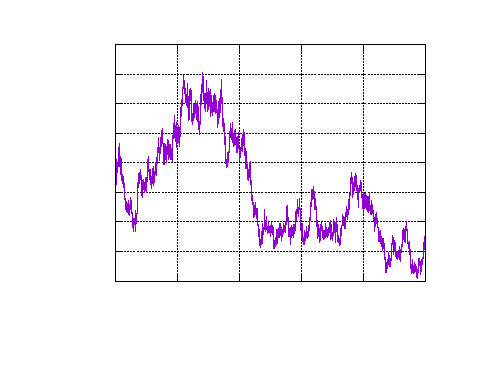
\includegraphics{Stock}}%
    \gplfronttext
  \end{picture}%
\endgroup

\caption{Sample stock data generated from \eqref{eq:geobrown}.}
\label{fig:stock}
\end{wrapfigure}

The goal of this project is to forecast stock prices using a deep neural network. While a daunting task, our first goal is to simulate a toy stock market in which we have total control of the parameters, and trends. This will better allow us to set up, train, test, and debug the neural network. \\

To do this we shall use the Black-Scholes model. In 1973 Fischer Black and Myron Scholes modelled stock prices with geometric Brownian motion, and Robert Merton extended its applicability. In 1997 they were awarded the Nobel Prize in Economics for their work. The price of a stock, $S_t$, is modelled by the stochastic differential equation
\begin{align}
dS_t &= \mu S_t dt + \sigma S_t dW_t,
\label{eq:sde}
\end{align}
where $W_t$ is a Wiener process. This can be discretized as
\begin{align}
S_{t+1} &= S_t \left( 1 + \mu \Delta t + \sigma \mathcal{N}(0,1) \sqrt{\Delta t} \right),
\label{eq:geobrown}
\end{align}
and this algorithm can easily be implemented, and an example of the result can be seen in Figure \ref{fig:stock}. From It\^{o} calculus the analytic solution to \eqref{eq:sde} is
\begin{align*}
S_t &= S_0 \exp \left( \left( \mu - \frac{1}{2} \sigma^2 \right) t + \sigma W_t \right)
\end{align*}
which may be useful for finding trends. \\

In probability theory, the characteristic function is an alternative representation of a probability distribution. The characteristic function, $\phi (\lambda)$, is given by $\mathbb{E} [\exp( i \lambda X_t) ]$, and as such is equal to the Fourier Transform of $X_t$. Working in the Fourier space provides a frequency representation of the stock prices, which may help remove the short-term noise in the prices and extract the long-term trends. \\

Generally, the characteristic function of a probability distribution is written in the form of the L\'{e}vy-Khintchine representation
\begin{align*}
\phi(\lambda) &= \exp \left(i \mu \lambda - \frac{\lambda^2 \sigma^2}{2} + \int_\mathbb{R} e^{i \lambda x} - 1 - i \lambda x 1_{\{ |x| < 1 \}} \nu(dx) \right).
\end{align*}
The first two terms come from Brownian motion with drift whereas the latter term comes from a Poisson jump. In the case $\nu = 0$, the last term vanishes and we simply obtain the characteristic function of the Black-Scholes model. With the characteristic function we have two different representations of the stock prices which we can use as a form of cross-validation for regression and classification. \\

Lastly, our final goal is to apply our neural network to real world stocks. The \texttt{pandas} package in Python includes functions to automatically pull financial data from Yahoo Finance which can then be divided into, for example, bi-weekly intervals and used to train and test the network. The Yahoo Finance data includes the daily high, low, open, and close prices, as well as the volume traded for each business day for the last five years. By looking at stocks within a particular industry, we should be able to obtain more than enough data in order to train the neural network. 
\end{document}
